% ALGUNOS PAQUETES REQUERIDOS (EN UBUNTU): %
% ========================================
% %
% texlive-latex-base %
% texlive-latex-recommended %
% texlive-fonts-recommended %
% texlive-latex-extra %
% texlive-lang-spanish (en ubuntu 13.10) %
% ******************************************************** %

\documentclass[a4paper]{article}
\usepackage[spanish]{babel}
\usepackage[utf8]{inputenc}
\usepackage{fancyhdr}
\usepackage[pdftex]{graphicx}
\usepackage{sidecap}
\usepackage{caption}
\usepackage{subcaption}
\usepackage{booktabs}
\usepackage{makeidx}
\usepackage{float}
\usepackage{amsmath, amsthm, amssymb}
\usepackage{amsfonts}
\usepackage{sectsty}
\usepackage{wrapfig}
\usepackage{listings}
\usepackage{pgfplots}
\pgfplotsset{compat=1.3}

\usepackage{fancyhdr}
\pagestyle{fancy}
%\renewcommand{\chaptermark}[1]{\markboth{#1}{}}
\renewcommand{\sectionmark}[1]{\markright{\thesection\ - #1}}
\fancyhf{}
\fancyhead[LO]{Sección \rightmark} % \thesection\
\fancyfoot[LO]{\small{Franco Frizzo, Iván Pondal, Manuel Mena, Maximiliano Paz}}
\fancyfoot[RO]{\thepage}
\renewcommand{\headrulewidth}{0.5pt}
\renewcommand{\footrulewidth}{0.5pt}
%\setlength{\hoffset}{-0.8in}
\setlength{\textwidth}{16cm}
\setlength{\hoffset}{-1.1cm}
\setlength{\headsep}{0.5cm}
\setlength{\textheight}{25cm}
\setlength{\voffset}{-0.7in}
\setlength{\headwidth}{\textwidth}
\setlength{\headheight}{13.1pt}
\renewcommand{\baselinestretch}{1.1} % line spacing

\usepackage{caratula}

\begin{document}
\materia{Algoritmos y Estructuras de Datos III}
\submateria{Primer Cuatrimestre de 2016}
\titulo{Trabajo Práctico I}
%\subtitulo{Grupo: }
\integrante{Franco Frizzo}{013/14}{francofrizzo@gmail.com}
\integrante{Iván Pondal}{078/14}{ivan.pondal@gmail.com}
\integrante{Manuel Mena}{xxx/xx}{xxx}
\integrante{Maximiliano Paz}{251/14}{m4xileon@gmail.com}
\maketitle
% no footer on the first page
\thispagestyle{empty}

\newpage
\tableofcontents

\newpage
\section{Introducción}

En este trabajo se tienen tres problemas que se resolvieron aplicando las
técnicas algorítmicas estudiadas en la materia. Los mismos presentaron cada uno un desafío
distinto, teniendo que aplicar métodos diferentes para resolverlos y cumplir
con los requisitos exigidos.

Además de la resolución de los mismos, se procedió a demostrar la correctitud de
cada implementación. Esto fue acompañado a su vez de una justificación de la
complejidad temporal.

Cada ejercició contó con su respectiva experimentación para corroborar que la
complejidad temporal teórica se cumpliera y en los casos donde el algoritmo
podía comportarse mejor, verlo reflejado de alguna manera.

Los experimentos contaron con diversas medidas para asegurar su efectividad de
las cuales las siguientes fueron iguales para los tres problemas:
\begin{itemize}
	\item{Sólo se midió el costo temporal de generar la solución, no
			de lectura y escritura del problema.}
	\item{Para la medición del tiempo se utilizó la librería \texttt{chronos}
			con unidad de tiempo en nanosegundos.}
	\item{Todas las pruebas se ejecutaron en los laboratiorios de la facultad.}
\end{itemize}


\newpage
\section{Ejercicio 1}
    % 1. Describir detalladamente el problema a resolver dando ejemplos del mismo y sus soluciones.
    \subsection{Descripción del problema}
		\begin{figure}[ht]
			\begin{center}
				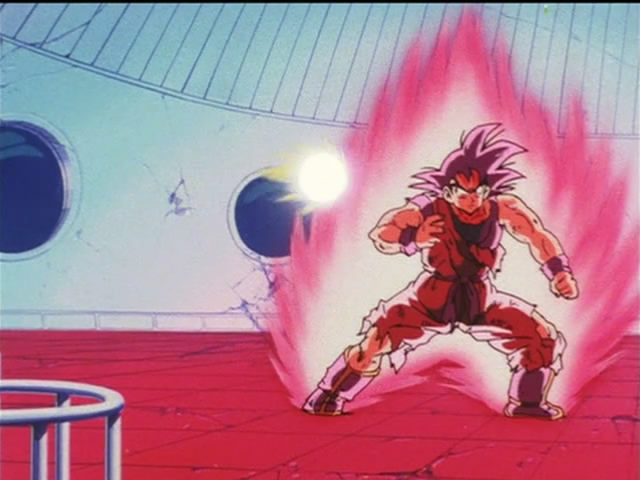
\includegraphics[width=0.5\columnwidth]{imagenes/kaioken.jpg}
				\caption{Los orígenes del CrossFit}
			\end{center}
		\end{figure}
        Gokú debe entrenar un ejército de $N$ guerreros para enfrentarse a Majin Boo. Para lograr ese objetivo, desea organizar peleas entre sus luchadores. En cada pelea, los guerreros serán divididos en dos bandos que pelearán entre sí. El objetivo es que, para cualquier par de luchadores, haya al menos una pelea en la que se encuentren en bandos distintos. Al mismo tiempo, el número total de peleas debe ser el mínimo necesario.

        La resolución del problema consiste en elaborar un programa que recibe como entrada el valor de $N$, y devuelve la cantidad mínima de peleas que deben llevarse a cabo para cumplir el cometido de Gokú y a continuación, por cada una de las peleas, una línea indicando el bando al que pertenece cada uno de los luchadores durante la misma. De haber más de una solución posible, puede devolverse cualquiera de ellas.

        Por ejemplo, si el programa recibe como entrada el valor \texttt{8}, cualquiera de las siguientes tres salidas sería correcta:

        \begin{center}\begin{tabular}{l @{\hskip 2em} | @{\hskip 2em} l @{\hskip 2em} | @{\hskip 2em} l}
            \texttt{3}               & \texttt{3}  &              \texttt{3}               \\
            \texttt{1 1 1 1 2 2 2 2} & \texttt{1 1 2 2 2 1 2 1} & \texttt{2 1 1 1 2 1 2 2} \\
            \texttt{1 1 2 2 1 1 2 2} & \texttt{1 1 2 1 2 2 1 2} & \texttt{1 2 1 1 2 2 2 1} \\
            \texttt{1 2 1 2 1 2 1 2} & \texttt{2 1 2 1 1 1 2 2} & \texttt{1 1 2 1 2 2 1 2} \\
        \end{tabular}\end{center}

    % 2. Explicar de forma clara, sencilla, estructurada y concisa, las ideas desarrolladas para la resolución del problema. Utilizar pseudocódigo y lenguaje coloquial (no código fuente). Justificar por qué el procedimiento resuelve efectivamente el problema.
    \subsection{Solución propuesta}
        La solución que se propone para el problema resulta más fácil de comprender con un sencillo cambio de óptica. En lugar de entender una solución como una sucesión de peleas, donde a cada una de ellas le corresponde una lista representando a un peleador, puede pensarse en una asignación entre cada guerrero y su \emph{historial de peleas}: la lista de los bandos que le fueron asignados en cada una de las peleas. Por ejemplo, si el historial de peleas de un guerrero es \texttt{2122}, esto significa que en la primera, la tercera y la cuarta pelea formó parte del bando número 2, mientras que en el segundo enfrentamiento peleó en el bando número 1. En una solución presentada según el formato requerido, los historiales de peleas de cada guerrero pueden verse si se la lee por columnas.

        Para que una solución al problema sea válida, es necesario cualquier par de peleadores diferentes se enfrente al menos en una pelea. Puede observarse que esto equivale a que el historial de peleas asignado a cada guerrero sea distinto, es decir, que difiera como mínimo en un dígito de todos los demás. Por otro lado, se pide que se lleve a cabo el mínimo número de peleas necesario, o lo que es lo mismo, que la longitud de los historiales de peleas sea la menor posible.

        Observando el problema desde esta perspectiva, es posible apreciar su semejanza con la construcción de un sistema de numeración posicional. Mientras que en un sistema de numeración se busca representar a los números naturales mediante una serie finita de símbolos provenientes de un alfabeto también finito, en una solución al problema planteado se busca asignar a cada peleador un historial de peleas, que consiste también en una serie finita de elementos de un conjunto finito: los bandos $1$ y $2$. Además, en un sistema de numeración, la representación de cada número tiene, en cierto sentido, la mínima longitud posible: estas se van asignando en orden creciente, y si queda ``libre'' una representación de cinco dígitos para un número, se utiliza esta antes que una de seis. Esto se parece al requisito de optimalidad requerido por el problema. Por último, dados dos números distintos, es necesario que sus representaciones en un sistema de numeración difieran como mínimo en un dígito, de forma análoga a lo que se desea que suceda con los historiales de peleas de dos guerreros diferentes.

        El sistema de numeración binario utiliza, comúnmente, los símbolos \texttt{0} y \texttt{1}. Sin embargo, esta elección es completamente arbitraria. Si se piensa en una variante de este sistema construida en base a los símbolos \texttt{1} y \texttt{2}, el problema de asignar un historial de peleas para $N$ guerreros que cumpla los requerimientos de Gokú puede reducirse a encontrar una representación en dicho sistema para los primeros $N$ números naturales. (A modo ilustrativo, pueden observarse las columnas de las soluciones de ejemplo expuestas en la descripción del problema. Si se reemplazan los símbolos $\lbrace\mathtt{1},\mathtt{2}\rbrace$ por $\lbrace\mathtt{0},\mathtt{1}\rbrace$, las columnas corresponden exactamente a la escritura binaria de los números entre $0$ y $7$).

        El algoritmo propuesto para resolver el problema planteado se basa en esta idea, y consiste simplemente en escribir los números naturales entre $0$ y $N-1$ en notación binaria utilizando $\lceil \log_2(N) \rceil$ dígitos para cada uno de ellos, pero cambiando los símbolos \texttt{0} y \texttt{1} por \texttt{1} y \texttt{2}, respectivamente. Estas escrituras representarán el historial de peleas de cada guerrero. Dado que para escribir los primeros $N$ naturales en notación binaria son necesarios exactamente $\lceil\log_2(N)\rceil$ dígitos, esta será la mínima cantidad de peleas necesarias para que todos los guerreros se enfrenten alguna vez entre sí. La línea correspondiente a la $i$-ésima pelea se obtiene tomando en orden los $i$-ésimos dígitos de las escrituras generadas; en otras palabras, leyendo las mismas ``por columnas''.

        El resultado así obtenido cumple con los requisitos necesarios para ser solución del problema. En efecto:
        \begin{itemize}
            \item Dados dos guerreros distintos, estos se enfrentan como mínimo en una pelea, ya que sus historiales de peleas (las escrituras binarias de sus respectivos índices) difieren al menos en un elemento.

            \item No existe una solución con menos peleas. Para ver esto, es importante notar que, dado cualquier $k \in \mathbb{N}$, se pueden generar como máximo $2^k$ escrituras binarias distintas de longitud $k$. En otras palabras, si Gokú hace que más de $2^k$ luchadores se enfrenten en $k$ peleas, habrá al menos dos de ellos que compartirán bando en todas las peleas.

            Consideremos, para cualquier cantidad de guerreros $N$, una serie de $k$ peleas, donde $k \leq \lceil \log_2(N) \rceil - 1$. En tal caso
            \[ 2^k \leq 2^{\lceil \log_2(N) \rceil - 1} = \frac{1}{2} 2^{\lceil \log_2(N) \rceil} < N\]
            dado que $ 2^{\lceil \log_2(N) \rceil}$ es la mínima potencia de dos mayor o igual que $N$. Como acaba de verse, esto significa que habrá al menos un par de guerreros que no se enfrentará nunca. Es decir, no existen soluciones válidas al problema con menos de $\lceil \log_2(N) \rceil$ peleas.
        \end{itemize}

        \subsubsection{Detalles implementativos}
            El algoritmo fue implementado en lenguaje C++. Para almacenar la solución, se recurre a la clase \texttt{vector}, proporcionada por la librería estándar del lenguaje.

            La ejecución consiste en un ciclo que se repite $\lceil \log_2(N) \rceil$ veces. La $i$-ésima iteración de este ciclo corresponde a la $i$-ésima pelea de la solución, y durante ella se construye la línea correspondiente a la misma, escribiendo repetidamente los símbolos \texttt{1} y \texttt{2}, alternando entre ellos cada $2^i$ símbolos. Es decir, la primera línea generada tiene la forma \texttt{1212121...}, la segunda, \texttt{1122112...}, y así sucesivamente. Si se observan las columnas del resultado así obtenido, se encuentran (con sus dígitos en orden inverso) las escrituras binarias de los primeros $N$ naturales, escritas con los símbolos \texttt{1} y \texttt{2}.

        \begin{codesnippet}
        \begin{verbatim}
cantidadPeleas = parte entera de log_2(n)
peleas = vector de tamaño cantidadPeleas inicializado en 2
saltos = 1
para i entre 0 y cantidadPeleas:
    para j entre 0 y n, con incrementos de 2 * saltos:
        para k entre 0 y saltos:
            si j + k < n:
                peleas[i][j + k] = 1
            fin si
        fin para
    fin para

    saltos = 2 * saltos
fin para

devolver peleas
        \end{verbatim}
        \end{codesnippet}

            En rigor, dado que la matriz necesaria para almacenar la solución es creada al comienzo de la ejecución, se aprovecha este momento para inicializarla con el símbolo \texttt{2}, utilizando el ciclo recién explicado para reemplazarlo por el símbolo \texttt{1} donde es necesario.

            % ¿MANDAMOS PSEUDOCÓDIGO? - NO, pero igual te quiero fran :) 

    % 3. Deducir una cota de complejidad temporal del algoritmo propuesto y justificar por qué el algoritmo cumple la cota dada. Utilizar el modelo uniforme.
    \subsection{Complejidad teórica}
         
      Durante la ejecución del algoritmo se utiliza una matriz con $\lceil \log_2(N) \rceil$ filas y $N$ columnas. En primer lugar, se inicializa esta matriz en \texttt{2}, lo cual tiene un costo del orden de $N \times \log(N)$. Para generar las peleas se recorre esta matriz; se tiene un ciclo que recorre las filas, y dentro del mismo, dos ciclos anidados que se encargan de recorrer las columnas. Los límites de estos últimos dos ciclos varían según la fila; en la fila $i$-ésima, el ciclo externo itera hasta $N$ con incrementos de tamaño $2^i$ ($\frac{N}{2^i}$ iteraciones), mientras que el ciclo interno itera hasta $2^i$ con saltos de a $1$ ($2^i$ iteraciones).

      Por lo tanto, la cantidad de veces que se ejecuta el ciclo interno, sumando sobre todas las filas de la matriz, es

      \[\sum_{i = 0}^{\log(N)} \sum_{j = 0}^{\frac{N}{2^i}} 2^i = \sum_{i = 0}^{\log(N)} \frac{N}{2^i} 2^i = \sum_{i = 0}^{log(N)} N = N \times \log(N)\]

      Como dentro de este último ciclo solo se modifica el valor de una posición de la matriz, con un costo $\ord(1)$, se puede concluir que la complejidad total del algoritmo es $\ord(N \times \log(N))$. 


    % 4. Dar un código fuente claro que implemente la solución propuesta. Se deben incluir las partes relevantes del código como apéndice del informe impreso entregado.

    % 5. Realizar una experimentación computacional para medir la performance del programa implementado. Usar un conjunto de casos de test en función de los parámetros de entrada, con instancias aleatorias e instancias particulares (de peor/mejor caso en tiempo de ejecución, por ejemplo). Presentar en forma gráfica una comparación entre los tiempos medidos y la complejidad teórica calculada y extraer conclusiones.
    \subsection{Experimentación}

	A la hora de medir el rendimiento del algoritmo y confirmar la complejidad
	teórica se tuvieron que considerar varios aspectos tales que los
	resultados de la experimentación reflejaran lo mejor posible su
	comportamiento.

	Dado que el problema consiste en una única entrada, los casos de prueba
	posibles se reducen al conjunto de los números enteros positivos. Como la
	complejidad temporal del algoritmo es $\theta(Nlog(N))$, no hay un peor
	y mejor escenario, por lo tanto no es necesario establecer condiciones sobre
	la entrada.

	El experimento consiste en la medición de los tiempos de ejecución para
	entradas cada vez más grandes. A continuación se describen las condiciones aplicadas
	para el mismo:

	\begin{itemize}
		\item{Como entrada se utilizó $N = k$ con $200 < k < 100000$}
		\item{Por cada $N$, se repitió 40 veces la medición y se calculó un
			promedio.}
	\end{itemize}

	De estos puntos, cabe destacar la elección de comenzar con $N = 200$. Esta
	decisión surge del hecho de que en valores pequeños las mediciones de tiempo
	son más sensibles a perturbaciones del sistema en el que están corriendo.
	Por lo tanto, en base a las pruebas realizadas, se optó por ignorar los
	primeros valores dado que no aportaban información pertinente al experimento.

	Los resultados obtenidos fueron los siguientes:

	\newcommand\constante{3}
	\begin{figure}[H]
		\centering
		\caption{}
		\label{fig:exp1:tiempo_base}
		\begin{tikzpicture}
			\begin{axis}[
					title={},
					xlabel={Tamaño de entrada ($N$)},
					ylabel={Tiempo de ejecución (nanosegundos)},
					scaled x ticks=false,
					scaled y ticks=false,
					enlargelimits=0.05,
					width=0.5\textwidth,
					height=0.5\textwidth,
					legend pos=south east,
					legend cell align=left,
					xmin=1
				]
				\addplot[color=black] table[x index=0,y index=1]{../exp/kaioKenOutput};
				\addplot[color=red] table[x index=0, y expr={x*ln(x)*\constante}]{../exp/kaioKenOutput};
				\legend{$T$, $c*N*log(N)$}
			\end{axis}
		\end{tikzpicture}
	\end{figure}

	En la Figura \ref{fig:exp1:tiempo_base} se puede observar como la curva generada por el
	tiempo de ejecución puede ser acotada para un $c$ fijo por una función
	$c*N*log(N)$. Para ratificar esta observación se procede dividiendo cada $T$
	por su respectivo $N$ con la intención de generar una curva de forma
	logarítmica.

	\begin{figure}[H]
		\centering
		\caption{}
		\label{fig:tiempo_sobre_n}
		\begin{tikzpicture}
			\begin{axis}[
					title={},
					xlabel={Tamaño de entrada ($N$)},
					ylabel={Tiempo de ejecución (nanosegundos)},
					scaled x ticks=false,
					scaled y ticks=false,
					ymax=100,
					enlargelimits=0.05,
					width=0.5\textwidth,
					height=0.5\textwidth,
					legend pos=south east,
					legend cell align=left,
					xmin=1
				]
				\addplot[color=black] table[x index=0,y index=2]{../exp/kaioKenOutput};
				\addplot[color=red] table[x index=0, y expr={ln(x)*\constante}]{../exp/kaioKenOutput};
				\legend{$\frac{T}{N}$, $c*log(N)$}
			\end{axis}
		\end{tikzpicture}
	\end{figure}

	Con la Figura \ref{fig:tiempo_sobre_n} se corrobora lo previsto, ya que
	efectivamente se puede apreciar cómo con la misma constante $c$ se puede
	acotar por una función $c*log(N)$.

	\begin{figure}[H]
		\centering
		\caption{}
		\label{fig:tiempo_sobre_n_log_n}
		\begin{tikzpicture}
			\begin{axis}[
					title={},
					xlabel={Tamaño de entrada ($N$)},
					ylabel={Tiempo de ejecución (nanosegundos)},
					scaled x ticks=false,
					scaled y ticks=false,
					ymin=0,
					ymax=5,
					enlargelimits=0.05,
					width=0.5\textwidth,
					height=0.5\textwidth,
					legend pos=south east,
					legend cell align=left,
					xmin=1
				]
				\addplot[color=black] table[x index=0,y index=3]{../exp/kaioKenOutput};
				\addplot[color=red] table[x index=0, y expr={\constante}]{../exp/kaioKenOutput};
				\legend{$\frac{T}{N*log(N)}$, $c$}
			\end{axis}
		\end{tikzpicture}
	\end{figure}

	Finalmente, en la Figura \ref{fig:tiempo_sobre_n_log_n} se tiene que
	$\frac{T}{N*log(N)}$ converge a una constante que puede ser acotada por $c =
	\constante$. Este $c$ es el mismo que es utilizado en las figuras
	anteriores.

	Es así como se llega a la conclusión de que efectivamente la complejidad
	temporal de la solución desarrollada coincide con la complejidad teórica estipulada.

	Para reproducir los datos utilizados basta con ejecutar \texttt{KaioKenSolver
	-p}.


\newpage

\section{Ejercicio 2}
    % 1. Describir detalladamente el problema a resolver dando ejemplos del mismo y sus soluciones.
    \subsection{Descripción del problema}
        $N$ soldados de Freezer estan parados en distintos puntos $(X_i,Y_i)$ sobre nuestro planeta y estan dispuestos a acabar con toda la humanidad. Para esto, Goku desea lanzarles algunas Genkidamas que puedan acabar con ellos. Los puntos cumplen con la propiedad $ X_1 > X_2 >. . . > X_N \geq 0 $ y $ 0 \leq Y_1 < Y_2 < . . . < Y_N$ . Goku quiere lanzar las Genkidamas a puntos donde hay enemigos, por lo que si en un punto no hay un enemigo no puede lanzar una Genkidama a ese punto (si puede lanzarla si habia un enemigo que ya fue destruido por Goku con una Genkidama previa). Una Genkidama lanzada al punto $(X,Y)$ destruye a todos los enemigos que estan en el rectangulo con lados paralelos a los ejes y extremos en $(0, 0)$ y $(X + T, Y + T )$

        Se pide escribir un algoritmo que tome el numero de enemigos de Goku, las posiciones de los mismos, y el valor de $T$ , y que indique la minima cantidad de Genkidamas debe lanzar Goku para acabar con todos sus enemigos, junto con los  indices de aquellos enemigos a cuyas posiciones lanza las Genkidamas. El algoritmo debe tener una complejidad temporal $O(N)$, siendo $N$ la cantidad de enemigos.

    % 2. Explicar de forma clara, sencilla, estructurada y concisa, las ideas desarrolladas para la resolución del problema. Utilizar pseudocódigo y lenguaje coloquial (no código fuente). Justificar por qué el procedimiento resuelve efectivamente el problema.
    \subsection{Solución propuesta}
        Si tirara un genkidama a cada enemigo eso solucionaria el problema de matar a todos los enemigos, pero solo seria solucion optima si todos los enemigos estuviesen a una distancia mayor a $\sqrt{2}T$ , ya que cada enemigo tendria una diferencia mayor a $T$ con respecto a las coordenadas $x$ e $y$. 

        Ahora si un enemigo esta a una diferencia con respecto a la coordenada $y$ menor a $T$ del enemigo siguiente , tirando una genkidama a ese enemigo y no al siguiente reduciria en uno la cantidad de genkidamas ha tirar. Si no , si el proximo enemigo esta a una diferencia menor a $T$ en con respecto a la coordenada $x$, podria no tirar una genkidama sobre ese enemigo dejandolo pendiente, y cuando ya no pueda matar al primer enemigo que deje pendiente , tirar una genkidama sobre ese, asi poder ahorarme esos pendientes enemigos. A partir de la ideas recien expuestas, Se pasa a explicar el algoritmo:  


        LLamaremos $maxY$ a el maximo $y$ que cubre el último genkidama, y $xPendiente$ a la coordenada $x$ del primer enemigo que deje pendiente ha eleminar con un futuro genkidama.
        Para el caso $n = 1$ se ha resuelto devolviendo el único elemento. Para $n > 2$: si el primer enemigo no se puede dejar pendiendte, osea que $x_0 > x_1  - T$, entonces se ha de tirar un genkidama a él y se ha de guardar el maximo $y$ que cubre el genkidama en $maxY$, si no se ha guardar el $x$ del enemigo en $xPendiente$. Para los casos mayores a 1 y menores a $n$ , Si el $maxY$ es menor a la cordenada $y$ del enemigo, entonces si un genkidama tirado a el siguiente enemigo no cubre al anterior, osea $x_i > x_{i+1} - T$,  entonces tiro un genkidama a él , actualizo el maxY e intancio $xPendiente$ en $0$, si no , si $xPendiente$ es $0$ entonces lo reemplazo por la coordenada $x$ del enemigo actual, si un genkidama tirado a el siguiente enemigo no cubre al $xPendiente$, osea  $xPendiente > x_{i+1} - T$, entonces tiro un genkidama a él , actualizo el maxY e intancio $xPendiente$ en $0$. Si el último enemigo no es cubierto por el último genkidama entonces se ha de tirar un genkidama sobre él.

        Quiero ver que expuesto algoritmo cumple cierta propiedad la cual me ayudara a probar correctitud del problema previamente descriptó . Llamaremos $P$ a la propiedad expresada en primer orden , $a$ el array de puntos tomados como input del algoritmo y $S$ el conjunto de enemigos a los cuales se tiraran genkdamas. 
         $P(a) = \forall_{(0 \leq i < n)} ( (i > 0) \land ( (a_i)_y > (a_{i - 1})_y + T ) ) \lor ( (i < n-1) \land  ( (a_i)_x < (a_{i + 1})_x - T ) ) )  \iff  a_i \in S^\complement  $
        Caso Base n = 1



       
    % 3. Deducir una cota de complejidad temporal del algoritmo propuesto y justificar por qué el algoritmo cumple la cota dada. Utilizar el modelo uniforme.
    \subsection{Complejidad teórica}
         
       

    % 4. Dar un código fuente claro que implemente la solución propuesta. Se deben incluir las partes relevantes del código como apéndice del informe impreso entregado.

    % 5. Realizar una experimentación computacional para medir la performance del programa implementado. Usar un conjunto de casos de test en función de los parámetros de entrada, con instancias aleatorias e instancias particulares (de peor/mejor caso en tiempo de ejecución, por ejemplo). Presentar en forma gráfica una comparación entre los tiempos medidos y la complejidad teórica calculada y extraer conclusiones.
    \subsection{Experimentación}


\newpage
\section{Ejercicio 3}
    % 1. Describir detalladamente el problema a resolver dando ejemplos del mismo y sus soluciones.
    \subsection{Descripción del problema}
        Gokú se está enfrentando a N androides y necesita destruirlos con la menor cantidad de Kamehamehas posibles. Los enemigos ode Gokú se encuentran en posiciones $(X_i , Y_i)$ y los Kamehameha recorren una semirrecta desde donde Gokú lo lance, en cualquier dirección que Gokú lo decida. ¿Cuántos Kamehamehas necesita Gokú para desturir a todos los androides del doctor Maki Gero? \\

        Se pide escribir un algoritmo que tome la cantidad de androides N y las posiciones $(X_i , Y_i)$ de los mismos y decida cuántos Kamehameha debe lanzar Gokú y a qué enemigos destruye con cada Kamehameha. Si hay más de una solución óptima, el algoritmo puede devolver cualquiera de ellas. Se pide utilizar la técnica de Backtracking y elaborar podas y estrategias para mejorar los tiempos de ejecución; éstas deberán estar apropiadamente documentadas en el informe. El algoritmo debe tener una complejidad temporal $O(N^{N+2})$ o mejor. \\

        La salida que el algoritmo debe retornar consiste en la cantidad de kamehamehas seguido de esa cantidad de lineas, donde cada una comienza con lacantidad de androides destruidos, seguido por los indices de dichos androides. \\

        Por ejemplo, para la entrada: \\

        \texttt{5}   \\
        \texttt{0 0} \\
        \texttt{0 1} \\
        \texttt{0 2} \\
        \texttt{1 2} \\
        \texttt{2 2} \\
        

    % 2. Explicar de forma clara, sencilla, estructurada y concisa, las ideas desarrolladas para la resolución del problema. Utilizar pseudocódigo y lenguaje coloquial (no código fuente). Justificar por qué el procedimiento resuelve efectivamente el problema.
    \subsection{Solución propuesta}
    La solución consiste en probar todas las combinaciones posibles de kamehamehas, y retornar la lista de kamehamehas de menor tamaño


       
    % 3. Deducir una cota de complejidad temporal del algoritmo propuesto y justificar por qué el algoritmo cumple la cota dada. Utilizar el modelo uniforme.
    \subsection{Complejidad teórica}
         
       

    % 4. Dar un código fuente claro que implemente la solución propuesta. Se deben incluir las partes relevantes del código como apéndice del informe impreso entregado.

    % 5. Realizar una experimentación computacional para medir la performance del programa implementado. Usar un conjunto de casos de test en función de los parámetros de entrada, con instancias aleatorias e instancias particulares (de peor/mejor caso en tiempo de ejecución, por ejemplo). Presentar en forma gráfica una comparación entre los tiempos medidos y la complejidad teórica calculada y extraer conclusiones.
    \subsection{Experimentación}


\end{document}
